\documentclass[14pt,a4paper]{extarticle}
%\documentclass[12pt,a4paper]{article}

\usepackage[utf8]{inputenc}
\usepackage[ukrainian]{babel}


\usepackage{amssymb}
\usepackage{physics}


\usepackage[active]{srcltx}
\usepackage[final]{pdfpages}

\usepackage[hidelinks]{hyperref}

\usepackage{verbatim}
%%%%%%%%%%%%%%%%%%%%%%%%%%%%%%%%%%%%%%%%%%%%%%%%%%%%%%%%%%%%%%%%%%
%\pagestyle{empty}                     %нумерацiя сторiнок i т.д.
\pagestyle{headings}                   %нумерацiя сторiнок вгорi зправа i т.д.
%\renewcommand{\baselinestretch}{1.5}   %мiжстрiчковий інтервал
%\parindent=7.5mm                      %абзацний відступ
 \righthyphenmin=2                     %перенос 2 останніх букв
 \pagenumbering{arabic}
 \tolerance=400
 \mathsurround=2pt
 \hfuzz=1.5pt
%%%%%%%%%%%%%%%%%%%%%%%%%%%%%%%%%%%%%%%%%%%%%%%%%%%%%%%%%%%%%%%%%%
 \hoffset=-0.5cm        %+2.5cm -- вiдступ вiд лiвого краю
 \voffset=-1.5cm        %+2.5cm -- вiдступ зверху
 \oddsidemargin=0.1cm   %ліве поле
 \topmargin=0.1cm       %верхнє поле
 \headheight=0.5cm      %висота верхнього колонтитулу
 \footskip=1cm          %висота нижнього колонтитулу
 \headsep=0.3cm         %відступ від колонт. до тексту
 \textwidth=17cm        %ширина сторінки
 \textheight=25.5cm     %висота сторінки
%%%%%%%%%%%%%%%%%%%%%%%%%%%%%%%%%%%%%%%%%%%%%%%%%%%%%%%%%%%%%%%%%%
 \newcounter{e}
 \setcounter{e}{0}
 \newcommand{\n}{\refstepcounter{e} (\arabic{e})}
 
 \newcounter{pic}
 \setcounter{pic}{0}
 \newcommand{\pic}[1]{\refstepcounter{pic} \vspace{-0.3cm}\textit{Рисунок \arabic{pic}\label{#1}.}}
 
 \newcounter{tabl}
 \setcounter{tabl}{0}
 \newcommand{\tabl}[1]{\refstepcounter{tabl} \vspace{-0.3cm}\textit{Таблиця \arabic{tabl}\label{#1}.}}
 
 \newcounter{dod}
 \setcounter{dod}{0}
 \newcommand{\dod}[1]{\refstepcounter{dod} \textit{Додаток \arabic{dod}\label{#1}.}}
 
% \newcounter{defn}
 %\setcounter{defn}{0}
 %\newcommand{\defn}[1]{\refstepcounter{defn} %\textbf{Означення \arabic{defn}\label{#1}.}}
 
 %\newcounter{theorem}
 %\setcounter{theorem}{0}
 %\newcommand{\theorem}[1]{\refstepcounter{theorem} %\textbf{Теорема \arabic{theorem}\label{#1}.}}
 \newtheorem{theorem}{Теорема}[section]
 \newtheorem{defn}[theorem]{Означення}
 \newtheorem{lemma}[theorem]{Лема}
 
 \newcommand{\proof}{\textit{Доведення. \space}}
% \setcounter{page}{1}
% \setcounter{section}{1}

\numberwithin{equation}{section}
\numberwithin{figure}{section}
%%%%%%%%%%%%%%%%%%%%%%%%%%%%%%%%%%%%%%%%%%%%%%%%%%%%%%%%%%%%%%%%%%
 \newcounter{stali}
 \setcounter{stali}{0}
 \newcommand{\s}{\refstepcounter{stali} \arabic{stali}}

 \newcommand{\st}{C_{\s}}
 \newcommand{\stl}[1]{C_{\s \label{#1}}}

 \newcommand{\cd}{{} $$ \vspace{-0.3cm} $$ {}}
 
 \newcommand{\nb}[2]{\righthyphenmin=#2 #1 \righthyphenmin=2}

%%%%%%%%%%%%%%%%%%%%%%%%%%%%%%%%%%%%%%%%%%%%%%%%%%%%%%%%%%%%%%%%%%
 
 \newcommand{\tabboxl}[2]{\parbox{#1}{\vspace{0.1cm} #2 \vspace{0.1cm} }}
 
 
 \newcommand{\tabboxr}[2]{\parbox{#1}{\vspace{-0.3cm}
 		\begin{flushright} #2 \end{flushright} \vspace{-0.3cm} }}
 
 \newcommand{\tabboxc}[2]{\parbox{#1}{\vspace{-0.3cm}
 		\begin{center} #2 \end{center} \vspace{-0.3cm} }}

 \newcommand{\liml}{\lim\limits}
 \newcommand{\suml}{\sum\limits}
 \newcommand{\intl}{\int\limits}
 
 \newcommand{\inttwopi}{\intl_{0}^{2\pi}}
 
 
%%%%%%%%%%%%%%%%%%%%%%%%%%%%%%%%%%%%%%%%%%%%%%%%%%%%%%%%%%%%%%%%%%
% bibliography
\usepackage[
backend=biber,
style=numeric,
sorting=none
]{biblatex}
\addbibresource{resources/bibliography.bibtex}
%%%%%%%%%%%%%%%%%%%%%%%%%%%%%%%%%%%%%%%%%%%%%%%%%%%%%%%%%%%%%%%%%%

 \begin{document}
	
 %\bibliographystyle{insrt}

 \thispagestyle{empty}

 \begin{center}
	\large
	Міністерство освіти і науки, молоді та спорту України \\
	Львівський національний університет імені Івана Франка \\
	Факультет прикладної математики та інформатики \\
	Кафедра обчислювальної математики
 \end{center}

 \vspace{45pt}

 \vfill

 \begin{center}
	{\Huge{Звіт}}\\
	{\large на тему:}
 \end{center}

 \begin{center}\Large
	\textbf{\emph{"Розв'язування задачі Діріхле-Неймана для рівняння Лапласа"}}
 \end{center}

 \vfill
 \vskip100pt

 \begin{flushleft}
	\hskip8cm 
	Виконали:
	\\ \hskip8cm 
	студенти IV курсу групи ПМп-41
	\\ \hskip8cm
	напрямку підготовки (спеціальності)
	\\ \hskip8cm
	113 -- ``Прикладна математика''
	\\ \hskip8cm
	Бугрій Б.О.
	\\ \hskip8cm
	Середович В.B.
 \end{flushleft}

 \begin{flushleft}
	\hskip8cm 
	Перевірили:
	\\ \hskip8cm
	проф. Хапко Р.С.
	\\ \hskip8cm
	ст. в. Гарасим Я.С.
 \end{flushleft}

 \vfill

 \begin{center}
	\large
	Львів - 2020
 \end{center}

 \newpage
 \thispagestyle{empty}
 \tableofcontents

 \newpage
 \thispagestyle{empty}
 \addcontentsline{toc}{section}{Вступ}
 \section*{Вступ}
 \begin{center}\end{center}
 літературний огляд \\
 хто розглядав розв'язування цієї задачі \\
 які процеси описує \\
 мета - розв'язати якимось методом \\
 огляд наступних розділів

 \newpage
 \thispagestyle{empty}
 \section{Постановка задачі}
		
	Припускаємо, що деяке двовимірне тіло задається двозв'язною областю $D \subset \mathbb{R}^2$ з досить гладкою границею що складається з внутрішньої кривої $\Gamma_1$ та зовнішньої $\Gamma_2$. 
	
	Нехай $D_1 \subset \mathbb{R}^2$ – обмежена область з гладкою границею $\Gamma_1 \subset C^2$ та $D_2 \subset \mathbb{R}^2$ – обмежена область з гладкою границею $\Gamma_2 \subset C^2$, причому $D_1\subset D_2$. Тоді двозв'язна область $D = D_2 \; \backslash \; \overline{D}_1$ матиме вигляд:

	\begin{figure}[h]
		\centering
		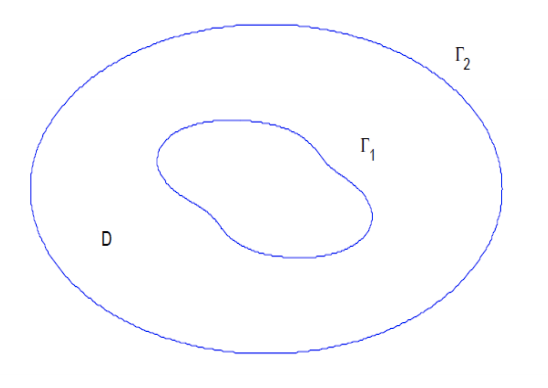
\includegraphics[width=0.55\textwidth]{resources/doubly-connected-region}
		\caption{}
		\label{fig:double-connected-region}
	\end{figure}

	Мішана задача Діріхле-Неймана для рівняння Лапласа полягає в знаходженні такої функції $u \in C^{2}(D)\cap  C^{1}(\overline{D})$ що задовольняє

	\begin{enumerate}
		\item
		Рівняння Лапласа: 
		\begin{equation}
			\label{laplace-eq}
			\Delta{u} = 0 \quad \text{в} \quad D
		\end{equation}

		\item
		Граничні умови:
		\begin{equation}
			\label{dirichlet-condition}
			u = f_1 \quad \text{на} \quad \Gamma_1,
			\vspace{-0.5cm}
		\end{equation}
	
		\begin{equation}
			\label{neumann-condition}
			\pdv{u}{\nu} = f_2 \quad \text{на} \quad \Gamma_2,		
		\end{equation}

	\end{enumerate}
	де $\nu = \nu(x)$ - одиничний вектор зовнішньої нормалі, (\ref{dirichlet-condition}) називають умовою Діріхле, а (\ref{neumann-condition}) -- умовою Неймана.
	
\newcommand{\boundprob}{(\ref{laplace-eq}) -- (\ref{neumann-condition})} 
	
	
 \newpage
 \thispagestyle{empty}
 \section{Коректність задачі}
 \subsection{Єдиність розв'язку задачі}
 \begin{theorem}
	 \label{green}
	 Нехай $D$ - область з межею $\partial D \in C^1$ i $\overrightarrow{\nu} -$ одиничний вектор зовнішньої нормалі до межі $\partial D$. Тоді для $u \in C^1(\overline{D})$ і $v \in C^2(\overline{D})$ має місце перша формула Гріна
	 \begin{equation}
	 	\intl_{D}(u \Delta v+grad u \cdot grad v) d x=\intl_{\partial D} u \frac{\partial v}{\partial \nu} d s
	 \end{equation}
 \end{theorem}
 \proof Див. \cite{kress2012linear}.
  
 \begin{theorem}
	\label{single-sol}
	Нехай $\Gamma_{1}, \Gamma_{2}$ -- гладкі границі, що належать класу $C^1$, обмежують двозв'язну область $D$. Тоді задача \boundprob \space має на $D$ не більше одного розв'язку.
 \end{theorem}
 \proof Від супротивного. Нехай $\exists u_1, u_2 \in C^{2}(\overline{D}): u_1 \neq u_2 $ -- два різні розв'язки задачі \boundprob. Запишемо цю задачу для функції $u^* = u_1 - u_2$:
 $$
 \Delta u^* = \Delta u_1 - \Delta u_2 = 0
 $$
 $$
 u^* = u_1 - u_2 = f_1 - f_1 = 0 \quad \text{на} \quad \Gamma_1
 $$
 $$
 \frac{\partial u^*}{\partial \nu}
 = \frac{\partial u_1}{\partial \nu} - \frac{\partial u_2}{\partial \nu}
 = f_2 - f_2 = 0 \quad \text{на} \quad \Gamma_2
 $$
 Застосуємо першу формулу Гріна з теореми \ref{green} при $u = v = u^*$:
 $$
 \intl_{D}(\operatorname{grad} u^*)^2 dx
 = \intl_{\partial D} u^* \frac{\partial u^*}{\partial \nu} dS
 - \intl_{D} u^* \Delta u^* dx
 $$
 Тут $\partial D = \Gamma_1 \cup \Gamma_2$. Так як $\Delta u^* = 0 $ в $D$, $u^*=0$ на $\Gamma_1$ і $\frac{\partial u^*}{\partial \nu} = 0$ на $\Gamma_2$, то отримуємо рівність
 $$
 \intl_{D}(\operatorname{grad} u^*)^2 dx = 0,
 $$
 з якої випливає, що $\frac{\partial u^*}{\partial x_1} = 0$ і $\frac{\partial u^*}{\partial x_2} = 0$ на всій області $D$, тобто $u^* = \operatorname{const}$. Функція $u^*$ неперервна в $\overline{D}$ і $u^*=0$ на $\Gamma_1 \subset \overline{D}$, отже $u^*\equiv0 \Rightarrow u_1\equiv u_2$, що суперечить початковому припущенню. $\blacksquare$
 
 \newpage
 \thispagestyle{empty}
 \section{Зведення до інтегрального рівняння}
 \subsection{Теорія потенціалів. Потенціал простого шару}

\begin{defn}
	\label{harminic-func}
	Нехай $D \subset \mathbb{R}^2$ -- замкнена обмежена область. Функція $u \in C^2(D)$, що набуває дійсних значень, називається гармонічною, якщо вона задовольняє рівняння Лапласа $\Delta u = 0$ в $D$.
\end{defn}

 \begin{defn}
	 \label{fundamental-solution}  
	 Функція
 	 \begin{equation}
		 \Phi(x, y) := \frac{1}{2\pi} \ln \frac{1}{\abs{x - y}} 
	 \end{equation}
	 визначена на  $x \neq y,$ $x \in \mathbb{R}^2$ називається фундаментальним розв'язком рівняння Лапласа. Для фіксованого $y \in \mathbb{R}^2$ вона є гармонічною в $\mathbb{R}^2 \backslash \{y\}$.
 \end{defn}
  
 \begin{defn}
	\label{single-layer-potential}
	 Нехай функція $\varphi \in C(\partial D),$ тоді
	 \begin{equation}
		 u(x):=\intl_{\partial D} \varphi(y) \Phi(x, y) d s(y), \quad x \in \mathbb{R}^{2} \backslash \partial D
	 \end{equation}
	 називають потенціалом простого шару з густиною $\varphi .$
 \end{defn}

 \begin{theorem}
 	 \label{potential-on-bound} 
	 Нехай $\partial D$ належить класу $C^{2}$ і $\varphi \in C(\partial D) .$ Тоді потенціал простого шару $u$ з густиною $\varphi$ неперервний на $\mathbb{R}^{2} .$ На границі області справджується рівність
	 \begin{equation}
		 u(x)=\intl_{\partial D} \varphi(y) \Phi(x, y) d s(y), \quad x \in \partial D
	 \end{equation}
	 де інтеграл існує і розуміється як невласний.
 \end{theorem}
 \proof Див. \cite{kress2012linear}.
 
 \begin{theorem}
 	 \label{potential-partial-derevative}
	 Нехай $\partial D$ належить класу $C^{2} .$ Тоді для потенціалу простого шару $u$ з неперервною густиною $\varphi$ маємо, що
	 \begin{equation}
		 \frac{\partial u_{\pm}}{\partial \nu}(x) =
		 \intl_{\partial D} \varphi(y) \frac{\partial \Phi(x, y)}{\partial \nu(x)} d s(y) \mp \frac{1}{2} \varphi(x),
		 \quad x \in \partial D
	 \end{equation}
	 де
	 \begin{equation}
	 	\frac{\partial u_{\pm}}{\partial v}(x):=\lim _{h \rightarrow+0} v(x) \cdot \operatorname{grad} u(x \pm h v(x))
	 \end{equation}
	 слід розуміти в сенсі рівномірної збіжності на $\partial D$ і інтеграл існує як невласний.
 \end{theorem}
 \proof Див. \cite{kress2012linear}.
 
 \subsection{Загальний вигляд розв'язку}
 
 Задача \boundprob \space зводиться до системи інтегральних рівнянь з двома невідомими функціями.
 Потенціал простого шару є гармонічною функцією, а отже їх сума також гармонічна.
 Тому розв'язок задачі \boundprob \space будемо шукати у вигляді суми потенціалів простого шару
 \begin{equation}
	 \label{potentials-sum-solution}
	 u(x) 
	 = \intl_{\Gamma_1} \varphi_1(y) \Phi(x, y) d s(y)
	 + \intl_{\Gamma_2} \varphi_2(y) \Phi(x, y) d s(y)
	 , \quad x \in D
 \end{equation}
 з невідомими густинами $\varphi_1 \in C(\Gamma_{1}) $, $\varphi_2 \in C(\Gamma_{2})$.
 
 Враховуючи інтегральне подання розв'язку, крайові умови та властивості потенціалу простого шару, для знаходження невідомих функцій отримаємо таку систему інтегральних рівнянь:
 
 \begin{equation}
 	\label{IE-system}
	 \left\{
	 \begin{array}{l}
	 	\displaystyle
	 	  \intl_{\Gamma_{1}} \varphi_1(y) \Phi(x, y) d s(y)
	 	+ \intl_{\Gamma_{2}} \varphi_2(y) \Phi(x, y) d s(y)
	 	= f_{1}(x), \quad x \in \Gamma_{1} 
	 	\\ [1cm]
	 	\displaystyle
	 	\frac{1}{2}\varphi_2(x)
	 	+ \intl_{\Gamma_{1}} \varphi_1(y) \frac{\partial \Phi(x, y)}{\partial \nu(x)} d s(y) +
	 	\\ [0.3cm]
	 	\displaystyle \qquad \qquad \qquad \qquad \quad
	 	+ \intl_{\Gamma_{2}} \varphi_2(y) \frac{\partial \Phi(x, y)}{\partial \nu(x)} d s(y)
	 	= f_{2}(x), \quad x \in \Gamma_{2}
 \end{array}\right.
 \end{equation}

 Потенціал простого шару не має стрибка, але він може виникнути при диференціюванні. В другій частині другого рівняння точка інтегрування та точка спостереження лежать на одній кривій, що і породжує стрибок. Варто звернути увагу на те, що стрибок розглядається на зовнішній границі (границі Неймана), отже він буде додатнім.
 
 \begin{comment}
 Розв'язок задачі \boundprob \space будемо шукати у вигляді потенціалу простого шару:
 $$
 u(x)=\intl_{\partial D} \varphi(y) \Phi(x, y) d s(y), \quad x \in \mathbb{R}^{2} \backslash \partial D
 $$
 Враховуючи інтегральне подання розв'язку, крайові умови та властивості потенціалу простого шару отримаємо таку систему інтегральних рівнянь:
 $$
 \left\{
 \begin{array}{l}
 \displaystyle \intl_{\Gamma_{1}} \varphi(y) \Phi(x, y) d s(y)=f_{1}(x), \quad x \in \Gamma_{1} 
 \\ [0.3cm]
 \displaystyle \varphi(x) + 2\intl_{\Gamma_{2}} \varphi(y) \frac{\partial \Phi(x, y)}{\partial \nu(x)} d s(y)=2f_{2}(x), \quad x \in \Gamma_{2}
 \end{array}\right.
 $$
 \end{comment}
  
 \newpage
 \thispagestyle{empty}
 \section{Параметризація}

 Припустимо, що кривi $\Gamma_{1}$ та $\Gamma_{2}$ заданi в параметричному виглядi:
\begin{equation}
	\label{parametrization}
	 \Gamma_{i} := \{ x_{i}(t) = (x_{i1}(t), x_{i2}(t)), \; t \in [ 0, 2\pi ] \} , \quad i = 1, 2
\end{equation}
де $x_{i} : \mathbb{R} \rightarrow \mathbb{R}^2$, $2\pi$ періодична $\forall{t} \; \abs{x'(t)} > 0$.

Нехай $\nu$ - одиничний вектор зовнішньої нормалі до кривої $\Gamma_{i}$, заданий як:
\begin{equation}
	\nu(x_i(t)) = \left(
	\frac{
		x'_{i2}(t)}{\abs{x'_{i}(t)}
	},
	- \frac{
	x'_{i1}(t)}{\abs{x'_{i}(t)}}
	\right)
\end{equation}

Обчислимо похідну по нормалі від фундаментального розв'язку
$$
\pdv{\Phi(x, y)}{\nu(x)} = -\frac{1}{2\pi} \pdv{\ln(r)}{r}\pdv{r}{\nu(x)}
$$

\indent де $r = \abs{x - y}$, отримаємо

\begin{equation}
	\pdv{\Phi(x, y)}{\nu(x)} = \frac{1}{2\pi} \frac{(y - x) \cdot \nu(x)}{r^2} 
\end{equation}


Перейдемо до параметризованої системи. Таким чином використовуючи параметризацію (\ref{parametrization}) та вище наведенні перетворення подамо систему (\ref{IE-system}) у параметризованому вигляді.
\begin{equation}
\label{IE-parametrized-with-specia}
	\left\{
	\begin{array}{l}
		\displaystyle
		\frac{1}{2\pi} \inttwopi \psi_1(\tau) K_{11}(t, \tau) d \tau
		+ \frac{1}{2\pi} \inttwopi  \psi_2(\tau) K_{12}(t, \tau) d \tau
		= g_{1}(t)
		\\ [0.3cm]
		\displaystyle
		\frac{\psi_2(t)}{2\abs{x'_{2}(t)) }}
		+ \frac{1}{2\pi} \inttwopi \psi_1(\tau) K_{21}(t, \tau) d \tau
		+ \frac{1}{2\pi} \inttwopi  \psi_2(\tau) K_{22}(t, \tau) d \tau
		= g_{2}(t)
	\end{array}\right.
\end{equation}
де $\displaystyle \psi_{i}(t) = \varphi(x_{i}(t)) \abs{x'_{i}(t)}, \; g_{i} = f_{i}(x_{i}(t)), \;  i  = 1, 2; \; t \in [0, 2\pi]$. \\[0.3cm]
Ядра матимуть вигляд:

$$
	\begin{array}{l}
		\displaystyle
		K_{11}(t, \tau) = \left.
			 \ln{\frac{1}{\abs{x - y}}}
		\right|_{
			{\small \parbox{20mm}{$ x = x_1(t)$ \\[-3pt] $y = x_1 ({\tau})$}}
		} \quad \quad, \quad t \neq \tau
		\\ [0.8cm]
		
		\displaystyle
		K_{12}(t, \tau) = \left.
			\ln{\frac{1}{\abs{x - y}}}
		\right|_{
			{\small \parbox{20mm}{$ x = x_1(t)$ \\[-3pt] $y = x_2 ({\tau})$}}
		}
		\\ [0.8cm]
		
		\displaystyle
		K_{21}(t, \tau) = \left.
			\frac{(y - x) \cdot \nu(x)}{r^2}
		\right|_{
			{\small \parbox{20mm}{$ x = x_2(t)$ \\[-3pt] $y = x_1 ({\tau})$}}
		}
		\\ [0.8cm]
		
		\displaystyle
		K_{22}(t, \tau) = \left.
			\frac{(y - x) \cdot \nu(x)}{r^2}
		\right|_{
			{\small \parbox{20mm}{$ x = x_2(t)$ \\[-3pt] $y = x_2 ({\tau})$}}
		} 
		, \quad t \neq \tau
	\end{array}
$$

В ядрах $K_{12}$, $K_{21}$ внаслідок параметризації точки $x$ та $y$ знаходяться на різних кривих, з чого випливає що ці ядра неперервні і при інтегруванні в них не виникають особливості.

У випадку $K_{11}$, $K_{22}$ обидві точки знаходяться на одній кривій і тому вони мають, відповідно, логарифмічну і сингулярну особливості при $t = \tau$. 

Для  виділення логарифмічної особливості виконаємо наступні перетворення з $K_{11}$:
$$
\begin{aligned}
	K_{11}(t, \tau) 
	&=
	\frac{1}{2} \ln \frac{1}{\left|x_{1}(t)-x_{1}(\tau)\right|^{2}} \pm \frac{1}{2} \ln \left(\frac{4}{e} \sin ^{2} \frac{t-\tau}{2}\right)=\\
	&=
	-\frac{1}{2} \ln \left(\frac{4}{e} \sin ^{2} \frac{t-\tau}{2}\right)+\frac{1}{2} \ln \frac{\frac{4}{e} \sin ^{2} \frac{t-\tau}{2}}{\left|x_{1}(t)-x_{1}(\tau)\right|^{2}}
\end{aligned}
$$

Отже, ядро $K_{11}$ можна записати у вигляді:

$$
	\displaystyle
	K_{11}(t, \tau) = {K_{11}}^{(1)} \ln \left(\frac{4}{e} \sin ^{2}  \frac{t-\tau}{2}\right)+{K_{11}}^{(2)}(t, \tau) \\
$$

де ядра ${K_{11}}^{(1)}$ і ${K_{11}}^{(2)}$ матимуть вигляд:

$$
	\displaystyle
	{K_{11}}^{(1)}(t, \tau) =-\frac{1}{2};
	\displaystyle
	\quad \text{та} \quad
	\displaystyle
	{K_{11}}^{(2)}(t, \tau) =\frac{1}{2} \ln{\frac{\frac{4}{e} \sin ^{2} \frac{t-\tau}{2}}{\left|x_{1}(t)-x_{1}(\tau)\right|^{2}}}, \quad t \neq \tau;
$$

Для того щоб доозначити ${K_{11}}^{(2)}$, знайдемо границю за правилом Лопіталя
$$
\lim _{\tau \rightarrow t} K_{11}{ }^{(2)}(t, \tau) = \lim _{\tau \rightarrow t} \ln \frac{\frac{4}{e} \sin ^{2} \frac{t-\tau}{2}}{\left|x_{1}(t)-x_{1}(\tau)\right|^{2}}=\ln \frac{\frac{4}{e} \frac{(t-\tau)^{2}}{4}}{\left|x_{1}^{\prime}(t)\right|^{2}(t-\tau)^{2}}=\ln \frac{1}{e\left|x_{1}^{\prime}(t)\right|^{2}}
$$
В результаті отримаємо:

\begin{equation}
	{K_{11}}^{(2)}(t, \tau) =
	\left\{
	\begin{array}{l}
		\displaystyle
		\frac{1}{2} \ln{\frac{\frac{4}{e} \sin ^{2} \frac{t-\tau}{2}}{\left|x_{1}(t)-x_{1}(\tau)\right|^{2}}}
		,\quad t \neq \tau
		\\ [1cm]
		
		\displaystyle
		\frac{1}{2} \ln \frac{1}{e\left|x_{1}^{\prime}(t)\right|^{2}}
		,\quad  \quad  \quad  \quad   t = \tau
	\end{array}
	\right.
\end{equation}
Доозначуємо ядро $K_{22}$. Знайдемо границю при $\tau \rightarrow t$

\begin{comment}
 $$
 K_{11}(t, \tau) = 
 \left\{
 \begin{array1}{l}
 	\displaystyle
	K_{11}(t, \tau) = \left.
	\ln{\frac{1}{\abs{x - y}}}
	\right|_{
		\small \parbox{20mm}{$ x = x_1(t)$ \\[-4pt] $y = x_1 ({\tau})$}
	}, \quad t \neq \tau \\
 	[1cm]

	\displaystyle

	, \quad t = \tau
 \end{array1}
 \right.
 $$
\end{comment}

$$
\lim_{\tau \rightarrow t } \pdv{\Phi(x_{2}(t), x_{2}(\tau))}{\nu(t)} =
\frac{  x''_{2}(\tau) \cdot \nu (x_2(t)) }{ 2\abs{ x'_{2}(t)}^2 } 
$$

Отримаємо наступне параметризоване подання ядра:
 \begin{equation}
	 K_{22}(t, \tau) = 
	 \left\{
	 \begin{array}{l}
		 \displaystyle
		 \frac{ \left( x_{2}(\tau) - x_{2}(t) \right) \cdot \nu (x_2(t)) }{ \abs{ x_{2}(t)-x_{2}(\tau) }^2 } 
		 ,\quad t = \tau
		 \\ [1cm]
	 
	 	\displaystyle
	 	\frac{  x''_{2}(t) \cdot \nu (x_2(t)) }{ 2\abs{ x'_{2}(t)}^2 } 
	 	,\quad \quad  \quad  \quad  \quad  t \neq \tau
	 \end{array}
	 \right.
 \end{equation}

Отже, система буде мати вигляд
\begin{equation}
	 \label{IE-parametrized}
	 \left\{
	 \begin{array}{l}
	 	\displaystyle
	 	\inttwopi \psi_1(\tau) \left\{ {K_{11}}^{(1)} (t, \tau) \ln{\left( \frac{4}{e} \sin^{2}{\frac{t - \tau}{2}} \right) } + {K_{11}}^{(2)} (t, \tau) \right\} d \tau +
	 	\\[0.3cm] \qquad \qquad \qquad \qquad \qquad \qquad \qquad
	 	\displaystyle
	 	+ \inttwopi \psi_2(\tau) K_{12}(t, \tau) d \tau
	 	= 2\pi g_{1}(t)
	 	\\ [0.3cm]
	 	
	 	\displaystyle
	 	\pi\frac{\psi_2(t)}{\abs{x'_{2}(t))}}
	 	+ \inttwopi \psi_1(\tau) K_{21}(t, \tau) d \tau
	 	+ \inttwopi \psi_2(\tau) K_{22}(t, \tau) d \tau
	 	= 2\pi g_{2}(t)
	 \end{array}\right.
\end{equation}
 
 Використовуючи параметризацію (\ref{parametrization}) можемо записати розв'язок мішаної задачі (\ref{potentials-sum-solution}) в параметризованому вигляді:
 \begin{equation} 
	 u(x)=\frac{1}{2 \pi} \int_{0}^{2 \pi} \psi_{1}(\tau) K_{1}(x, \tau) d \tau+\frac{1}{2 \pi} \int_{0}^{2 \pi}  \psi_{2}(\tau) K_{2}(x, \tau) d \tau, \quad x \in D
 \end{equation}
 де відповідні ядра $K_{1}$ і $K_{2}$ мають вигляд:
 \begin{equation}
  	K_{1}(x, \tau)=\ln \frac{1}{\left|x-x_{1}(\tau)\right|}
  	\quad \text{та} \quad 
 	K_{2}(x, \tau)=\ln \frac{1}{\left|x-x_{2}(\tau)\right|}
 \end{equation}
 
 
 
 
 \newpage
 \thispagestyle{empty}
 \section{Чисельне розв'язування}
 
 \subsection{Метод колокації}
 Метод колокації належить до проекційних методів розв'язування лінійних інтегральних рівнянь. Ми будемо використовувати колокацію на основі поділу області $D$ на деякі підобласті, на яких шукана функція апроксимується алгебраїчними поліномами невисокого степеня, в нашому випадку кусково лінійними.
 
 Нехай
 \begin{equation}
 	\label{tabulation}
 	t_{j}=a+j h, \quad j=0, \ldots, n
 \end{equation} 
 це рівновіддалений поділ відрізка $[a, b]$ з кроком $h=(b-a) / n$. $X_{n} $ -- простір функцій, неперервних на $[a, b]$, звуження яких на підінтервал $[t_{j-1}, t_{j}]$ -- лінійна функція.
 
 Очевидно, що $\dim X_n = n+1$ і базис Лагранжа в цьому просторі має вигляд
 \begin{equation}
	 \label{basis}
	 \ell_{j}(t)=\left\{
	 \begin{array}{lc}
	 	\displaystyle
	 	\frac{t-t_{j-1}}{h}, \quad t \in\left[t_{j-1}, t_{j}\right], \quad j \geq 1 \\
	 	\displaystyle
	 	\frac{t_{j+1}-t}{h}, \quad t \in\left[t_{j}, t_{j+1}\right], \quad j \leq n-1 \\
	 	0, \qquad\qquad \text { в інших випадках }
	 \end{array}\right.
 \end{equation}
 з очевидним уточненням для $\ell_0$ та $\ell_n$.
 Шукані функції з системи (\ref{IE-parametrized}) подамо у вигляді суми
 \begin{equation}
 	\tilde{\psi_k}(t)=\sum_{j=1}^{n} c^{(k)}_{j} \ell_{j}(t), \quad k = 1,2
 \end{equation}
 Підставивши їх у систему (\ref{IE-parametrized}) отримаємо:
 
 \begin{equation}
	 \label{coll-sys}
	 \left\{
	 \begin{array}{l}
	 	\displaystyle
	 	  \sum_{j=1}^{n} c^{(1)}_{j} \inttwopi \ell_{j}(\tau) K_{11}(t, \tau) d \tau
	 	+ \sum_{j=1}^{n} c^{(2)}_{j} \inttwopi \ell_{j}(\tau) K_{12}(t, \tau) d \tau
	 	= 2\pi g_{1}(t)
	 	\\ [0.3cm]
	 	
	 	\displaystyle
	 	  \sum_{j=1}^{n} c^{(1)}_{j} \inttwopi \ell_{j}(\tau) K_{21}(t, \tau) d \tau +
	 	\\ [0.3cm]
	 	
	 	\displaystyle
	 	\qquad \qquad \quad
	 	+ \sum_{j=1}^{n} c^{(2)}_{j} \left\{
	 	      \pi \frac{\ell_{j}(t)}{\abs{x'_{2}(t)}}
	 	    + \inttwopi \ell_{j}(\tau) K_{22}(t, \tau) d \tau
	 	  \right\}
	 	= 2\pi g_{2}(t)
	 \end{array}\right.
 \end{equation}
 
 Цю систему необхідно протабулювати на основі рівновіддаленого поділу (\ref{tabulation}) по змінній t щоб знайти відповідні значення векторів $c^{(1)}$ і $c^{(2)}$.
 Подамо отримані результати в зручному матричному вигляді
 $$
 Ac=g
 $$
 де
 $$
 A =
 \begin{pmatrix}
	 \begin{matrix}
	 	G^{(1)}_{11} & \dots  & G^{(1)}_{1n} \\
	 	\vdots 		 & \ddots & \\
	 	G^{(1)}_{n1} & 		  & G^{(1)}_{nn} \\
	 \end{matrix} &
	 \begin{matrix}
	 	G^{(2)}_{11} & \dots  & G^{(2)}_{1n} \\
	 	\vdots 		 & \ddots & \\
	 	G^{(2)}_{n1} & 		  & G^{(2)}_{nn} \\
	 \end{matrix} \\[1cm]
	 \begin{matrix}
		G^{(3)}_{11} & \dots  & G^{(3)}_{1n} \\
		\vdots 		 & \ddots & \\
		G^{(3)}_{n1} & 		  & G^{(3)}_{nn} \\
	 \end{matrix} &
	 \begin{matrix}
		G^{(4)}_{11} & \dots  & G^{(4)}_{1n} \\
		\vdots 		 & \ddots & \\
		G^{(4)}_{n1} & 		  & G^{(4)}_{nn} \\
	 \end{matrix} \\
 \end{pmatrix}
 c = 
 \begin{pmatrix}
	c^{(1)}_1\\
	\vdots\\
	c^{(1)}_n\\[0.5cm]
	c^{(2)}_1\\
	\vdots\\
	c^{(2)}_n\\
 \end{pmatrix}
 g = 
 \begin{pmatrix}
	2\pi g_{11}\\
	\vdots\\
	2\pi g_{1n}\\[0.5cm]
	2\pi g_{21}\\
	\vdots\\
	2\pi g_{2n}\\
 \end{pmatrix}
 $$
 де
 $$
 \begin{matrix}
	G^{(1)}_{ji} = \inttwopi \ell_{j}(\tau) K_{11}(t_i, \tau) d \tau & \hspace{-1.7cm}
	G^{(2)}_{ji} = \inttwopi \ell_{j}(\tau) K_{12}(t_i, \tau) d \tau \\[1cm]
	G^{(3)}_{ji} = \inttwopi \ell_{j}(\tau) K_{21}(t_i, \tau) d \tau & \hspace{1cm}
	G^{(4)}_{ji} = \pi\frac{\ell_{j}(t_i)}{\abs{x'_{2}(t_i))}}
				 + \inttwopi \ell_{j}(\tau) K_{22}(t_i, \tau) d \tau \\
 \end{matrix}
 $$
 
 Опираючись на властивості базису (\ref{basis}), інтеграли в системі (\ref{coll-sys}) можна подати у спрощеному вигляді:
 
 \begin{equation}
 	\begin{matrix}
 	\displaystyle
 	\inttwopi \ell_{j}(\tau) K\left(t_{i}, \tau\right) d \tau=\frac{1}{h} \intl_{t_{j-1}}^{t_{j}}\left(\tau-t_{j-1}\right) K\left(t_{i}, \tau\right) d \tau + \\
 	\displaystyle
 	+\frac{1}{h} \intl_{t_{j}}^{t_{j+1}}\left(t_{j+1}-\tau\right) K\left(t_{i}, \tau\right) d \tau
 	\end{matrix}
 \end{equation}
 де $K$ -- одне із ядер.
 
 Тоді отримаємо такий вигляд наближеного розв'язку:

 \begin{equation}
 	\begin{matrix}
 	\displaystyle
 	\hspace{-1.5cm} u_n(x) = \frac{1}{2 \pi} \sum_{j=1}^{n} c^{(1)}_{j} \inttwopi \ell_{j}(\tau) K_{1}(x, \tau) d \tau + \\
 	\displaystyle
 	\hspace{1.5cm} + \frac{1}{2 \pi} \sum_{j=1}^{n} c^{(2)}_{j} \inttwopi \ell_{j}(\tau) K_{2}(x, \tau) d \tau, \quad x \in D
    \end{matrix}
 \end{equation}
 
 
 \subsection{Дискретизація}
 Метод колокації є частково дискретним методом, що означає що інтеграли в системі рівнянь можемо обчислити точно. На жаль, це не завжди вдається, тому в даній роботі ми дискретизуємо метод використавши квадратури.

Для обчислення ядра $K_{11}$ будемо використовувати відповідну квадратурну формулу. Для цього задаємо рівномірне розбиття:

$$
t_{i}:=i \pi / M, \quad i=0, \ldots, 2 M-1, M \in N
$$
Квадратурна формула буде мати вигляд:
\begin{eqnarray}
	\frac{1}{2 \pi} \inttwopi f(\tau) \ln \left(\frac{4}{e} \sin ^{2} \frac{t-\tau}{2}\right) d \tau \approx \sum_{j=0}^{2 M-1} R_{j}(t) f\left(t_{j}\right)
\end{eqnarray}
з ваговою функцією

\begin{equation}
	R_{j}(t):=-\frac{1}{2 M}\left\{1+2 \sum_{m=1}^{M-1} \frac{1}{m} \cos m\left(t-t_{j}\right)+\frac{\cos \left(t-t_{j}\right)}{M}\right\}
\end{equation} 

 Решта ядер не містять у собі особливості, тим більше легко бачити що вони є щонайменше двічі неперервно диференційовні на заданих кривих, отже доцільно буде для обчислення інтегралів застосувати квадратури трапецій:
 \begin{equation}
 	\displaystyle
 	\inttwopi f(\tau) d \tau \approx h \left(\frac{f(0)+f(2\pi)}{2}+\sum_{i=1}^{n-1} f\left(t_{i}\right)\right).
 \end{equation}
 
 
 \subsection{Похибка}
 
\begin{theorem}
	\label{collocation-error}
	Нехай $A: X \rightarrow X$ - обмежений лінійний оператор у банаховому просторі $X$ та $ (I-A):X \rightarrow X$ -- ізоморфізм. Припустимо, що $\left\|P_{n} A-A\right\| \rightarrow 0, n \rightarrow \infty .$ Тоді для достатньо великого $n \geq \mathbb{N}$ оператори $\left(I-P_{n} A\right)^{-1}: X \rightarrow X$ існують і є рівномірно обмежені. Для точного і наближеного розв'язку $\varphi-\varphi_{n}=\left(I-P_{n} A\right)^{-1}\left(\varphi-P_{n} \varphi\right)$ має місце двостороння оцінка
 \begin{equation}
	 \frac{1}{\left\|I-P_{n} A\right\|}\left\|\varphi-P_{n} \varphi\right\| \leq\left\|\varphi-\varphi_{n}\right\| \leq\left\|\left(I-P_{n} A\right)^{-1}\right\|\left\|\varphi-P_{n} \varphi\right\|
 \end{equation}
\end{theorem} 
Проекційний оператор визначається як
\begin{equation}
 \left(P_{n} \varphi\right)(x)= \sum_{j=0}^{n} \varphi\left(x_{i}\right) l_{j}(x) .
\end{equation}
 Для оператора $P_{n} \varphi$ маємо такі оцінки похибки
 $$
 \begin{array}{l}
 	\displaystyle
	\varphi \in C^{2}[a, b], \quad \left\|P_{n} \varphi-\varphi\right\|_{\infty} \leq \frac{1}{8} h^{2}\left\|\varphi^{\prime \prime}\right\|_{\infty}  
	\\[0.3cm]
 	
 	\displaystyle
	\varphi \in C[a, b], \quad \; \left\|P_{n} \varphi-\varphi\right\|_{\infty} \leq w(\varphi, h) \rightarrow 0
	\\[0.3cm]	
\end{array}
 $$
 Звідси 
 $$ 
 P_{n} \varphi \rightarrow \varphi,  \quad  \varphi \in C[a, b]
 $$
 
 Для відповідного інтегрального оператора $A: C[a, b] \rightarrow C[a, b]$ маємо $\left\|P_{n} A-A\right\| \rightarrow 0, n \rightarrow \infty$.
 Отже, можемо використовувати результати теореми (\ref{collocation-error}) для нашого випадку.

 Таким чином для достатньо великого $n \geq N$ апроксимаційне рівняння колокації $\left(I-P_{n} A\right) \varphi_{n}=P_{n} f$ має єдиний розв'язок:
\begin{equation}
	\varphi \in C[a, b], \quad \left\|\varphi_{n}-\varphi\right\|_{\infty} \leq M\left\|P_{n} \varphi-\varphi\right\|_{\infty}
\end{equation}
\begin{equation}
	\varphi \in C^{2}[a, b], \quad \left\|\varphi_{n}-\varphi\right\|_{\infty} \leq M \frac{1}{8} h^{2}\left\|\varphi^{\prime \prime}\right\|_{\infty}
\end{equation}
де М є деякою константою яка залежить від ядер системи.

 \newpage
 \thispagestyle{empty}
 \section{Чисельні експерименти} 
\subsection{Приклад 1}
Нехай криві $\Gamma_{1}$ та $\Gamma_{2}$ мають таке параметричне задання:
\begin{equation}
	\label{ex-curves}
	\begin{array}{l}
		\displaystyle
		\Gamma_{1}=\left\{x_{1}(t)=(0.9 \cos t, 0.9 \sin t), \quad t \in[0,2 
		\pi]\right\} \\
		
		\displaystyle
		\Gamma_{2}=\left\{x_{2}(t)=(2 \cos t, 2 \sin t), \quad  t \in[0,2 \pi]\right\} \\[0.1cm]
	\end{array}
\end{equation}

\begin{equation}
	\begin{array}{cr}
		\label{ex1}
		\displaystyle
		u = x, \quad (x, y) \in D   \\ [0.3cm]
		
		\displaystyle
		f_1 = x  \text { на } \Gamma_{1}
		\quad  \text {і}  \quad
		f_2 = 1  \text { на } \Gamma_{2} \quad
	\end{array}
\end{equation}

\begin{figure}[h]
	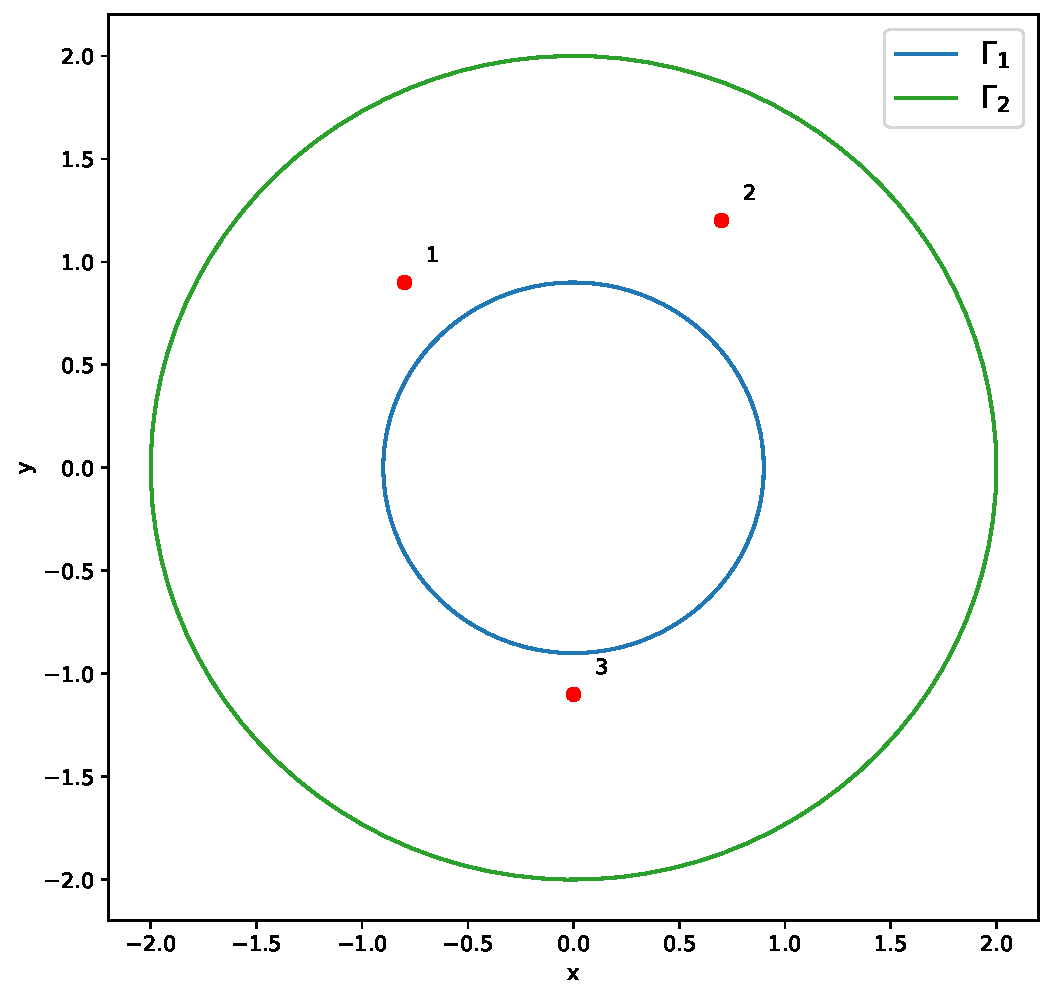
\includegraphics[width=0.4\textwidth]{resources/curves_and_points.pdf}
	\centering
	\caption{Граничні умови $\Gamma_1$, $\Gamma_2$ для (\ref{ex-curves})}
\end{figure}

В Табл. 1 наведено значення абсолютної похибки розв’язку мішаної задачі (\ref{laplace-eq}) - (\ref{neumann-condition}) в деяких точках $x \in D$ в залежностi вiд кiлькостi точок колокації $n$.

\begin{table}[h]
	\begin{center}
		\begin{tabular}{|c|c|c|c|}
			\hline
			
			\tabboxc{2cm}{n}     
			& \tabboxc{3cm}{x = (-0.8,0.9)}
			& \tabboxc{3cm}{x = (0.7,1.2)}
			& \tabboxc{3cm}{x = (-1, -1)}
			\\ \hline
			
			4
			& $1.54 \times 10 ^{-1}$
			& $1.57 \times 10 ^{-1}$
			& $3.25 \times 10 ^{-1}$
			\\ \hline
			8
			& $3.57 \times 10 ^{-2}$
			& $9.81 \times 10 ^{-2}$
			& $7.77 \times 10 ^{-2}$
			\\ \hline
			16
			& $4.98 \times 10 ^{-3}$
			& $2.67 \times 10 ^{-2}$
			& $9.52 \times 10 ^{-3}$
			\\ \hline
			32
			& $1.67 \times 10 ^{-4}$
			& $1.11\times 10 ^{-2}$
			& $2.11\times 10 ^{-3}$
			\\ \hline
		\end{tabular}
		\caption{Абсолютна похибка розв`язку}
	\end{center}
\end{table}

\begin{figure}[!htb]
	\minipage[t]{0.5\textwidth}
	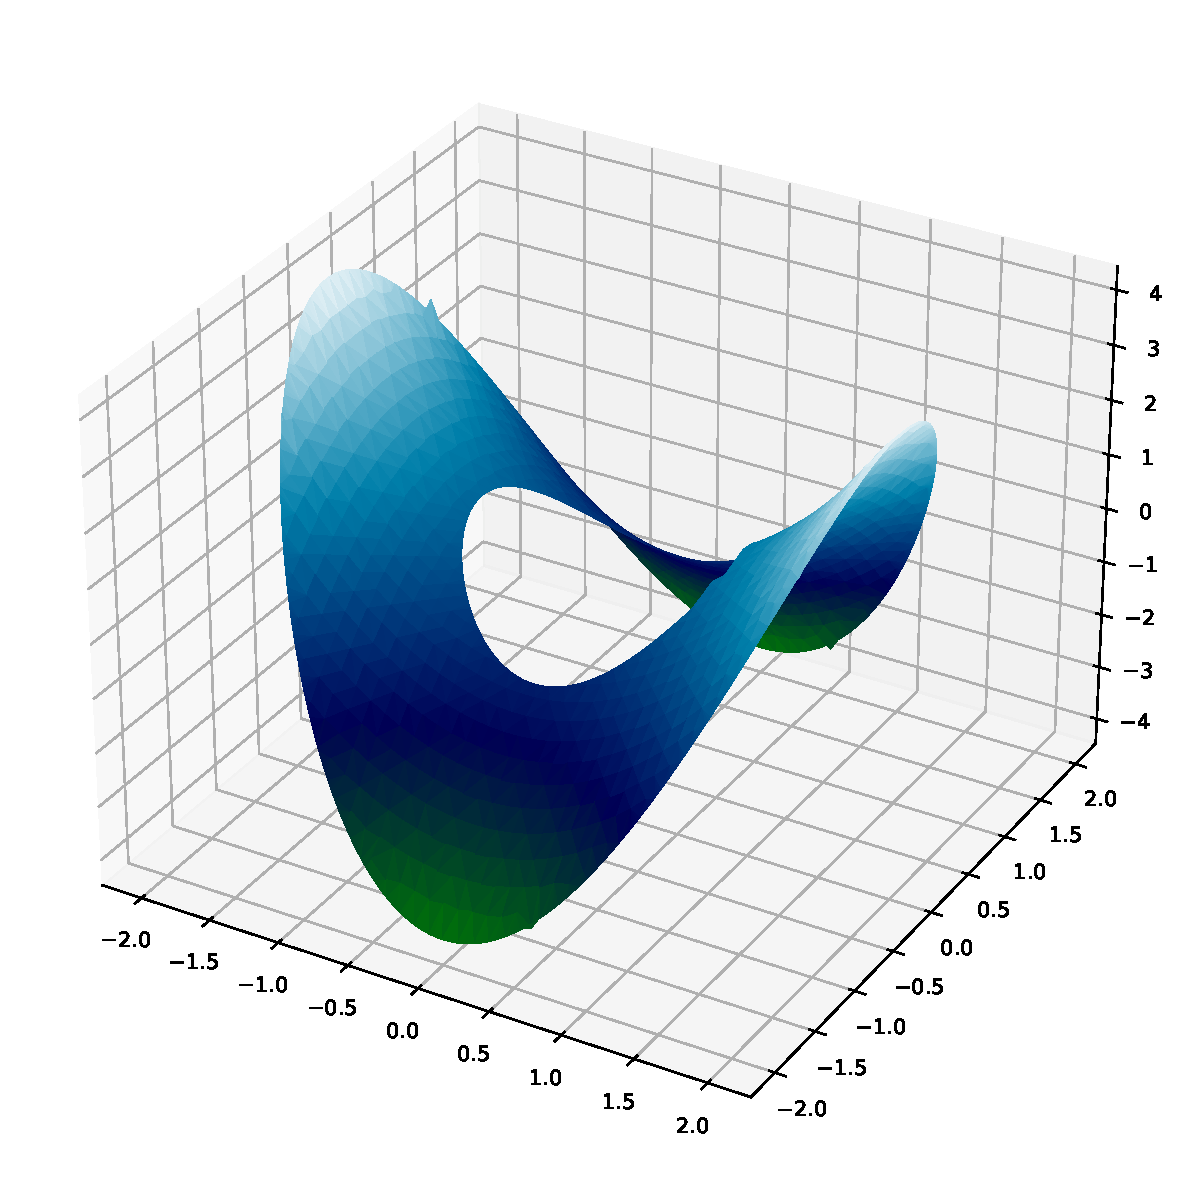
\includegraphics[width=1\textwidth]{resources/ex1-approx.pdf}
	\caption{Наближений розв'язок}
	\label{fig:ex1-approx}
	\endminipage
	\minipage[t]{0.5\textwidth}
	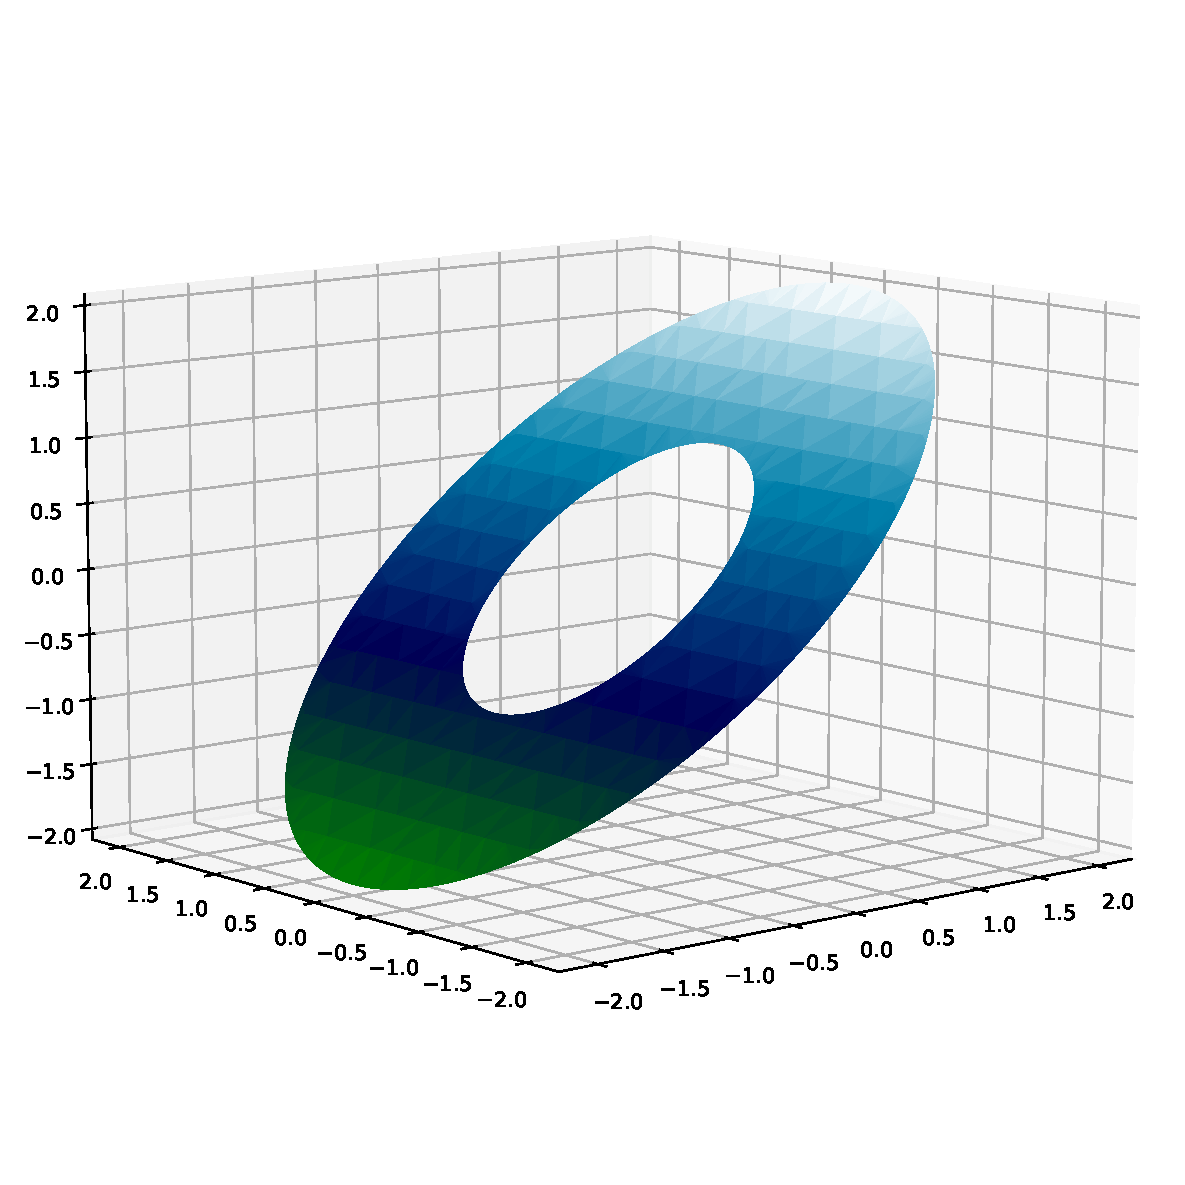
\includegraphics[width=1\textwidth]{resources/ex1-ex.pdf}
	\caption{Точний розв'язок}	
	\label{fig:ex1-exact}
	\endminipage\hfill
\end{figure}

\begin{figure}[!htb]
	\centering
	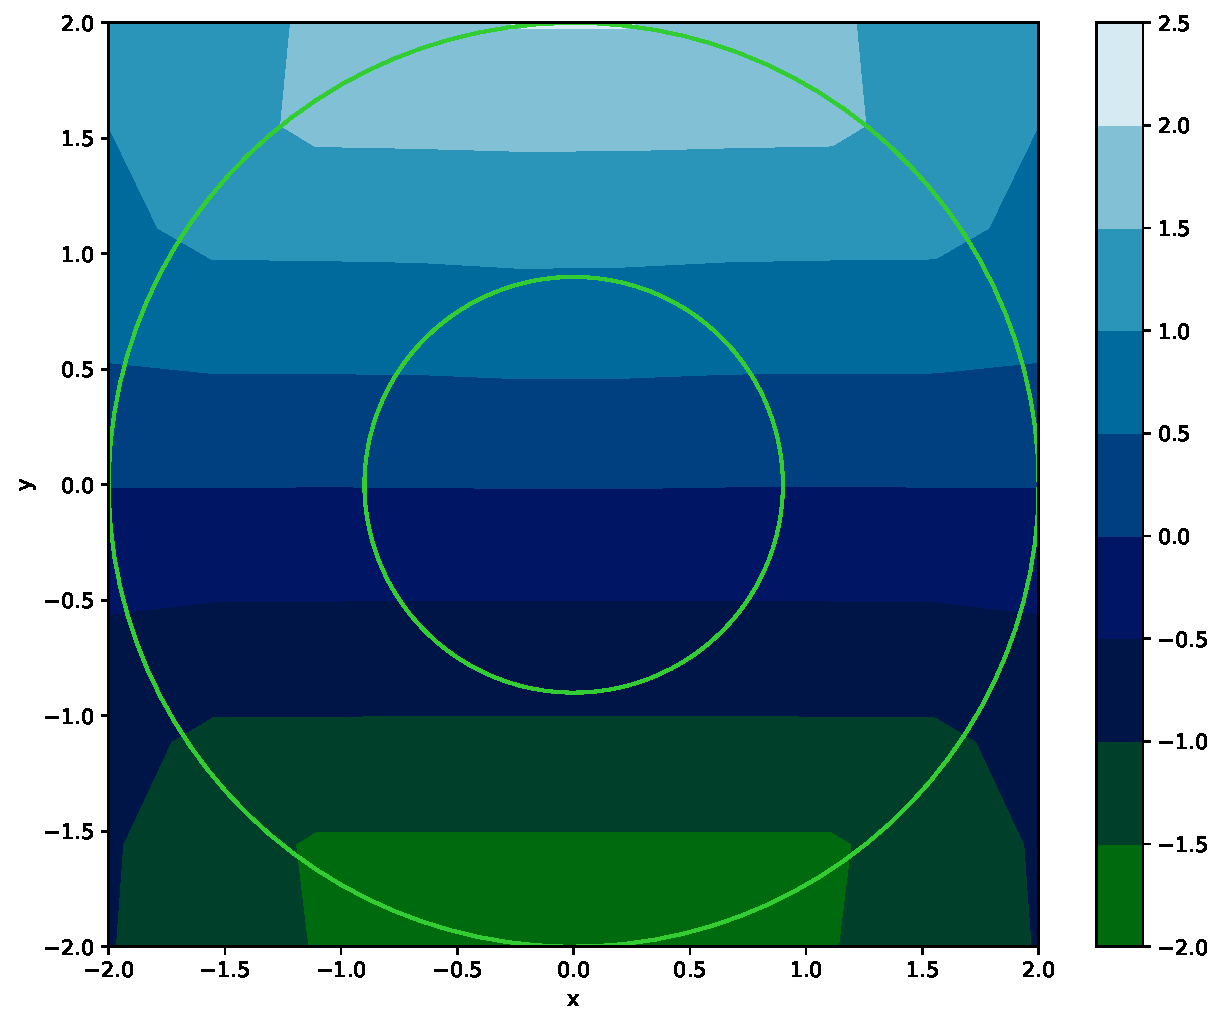
\includegraphics[width=0.45\textwidth]{resources/ex1_contourf.pdf}
	\caption{Лінії рівня наближеного розв'язку}
	\label{fig:ex1_contourf}
\end{figure}

 \newpage
 \subsection{Приклад 2}
  Розглянемо інший приклад для параметричного задання (\ref{ex-curves}).
\begin{equation}
	\label{ex2}
	\begin{array}{cr}
		\displaystyle
		u = x^2 - y^2, \quad (x, y) \in D \\[0.3cm]
		\displaystyle
		f_1 = x^2 - y^2  \text { на } \Gamma_{1}
		\quad  \text {і}  \quad
		f_2 = 2x - 2y \text { на } \Gamma_{2} \quad
	\end{array}
\end{equation}
 
 \begin{table}[h]
 	\begin{center}
 		\begin{tabular}{|c|c|c|c|}
 			\hline
 			
 			\tabboxc{2cm}{n}     
 			& \tabboxc{3cm}{x = (0.7,1.2)}
 			& \tabboxc{3cm}{x = (-0.8,0.9)}
 			& \tabboxc{3cm}{x = (-1, -1)}
 			\\ \hline
 			
 			4
 			& $3.32 \times 10 ^{-1}$
 			& $7.88 \times 10 ^{-2}$
 			& $3.11 \times 10 ^{-1}$
 			\\ \hline
 			8
 			& $1.07 \times 10 ^{-1}$
 			& $2.64 \times 10 ^{-2}$
 			& $4.91 \times 10 ^{-3}$
 			\\ \hline
 			16
 			& $5.30 \times 10 ^{-2}$
 			& $5.76 \times 10 ^{-3}$
 			& $8.18 \times 10 ^{-5}$
 			\\ \hline
 			32
 			& $1.44\times 10 ^{-2}$
 			& $2.48 \times 10 ^{-3}$
 			& $1.61\times 10 ^{-5}$
 			\\ \hline
 		\end{tabular}
 		\caption{\label{ex1-table} Абсолютна похибка розв`язку}
 	\end{center}
 \end{table}
 
 \begin{figure}[!htb]
  	\minipage[t]{0.5\textwidth}
	 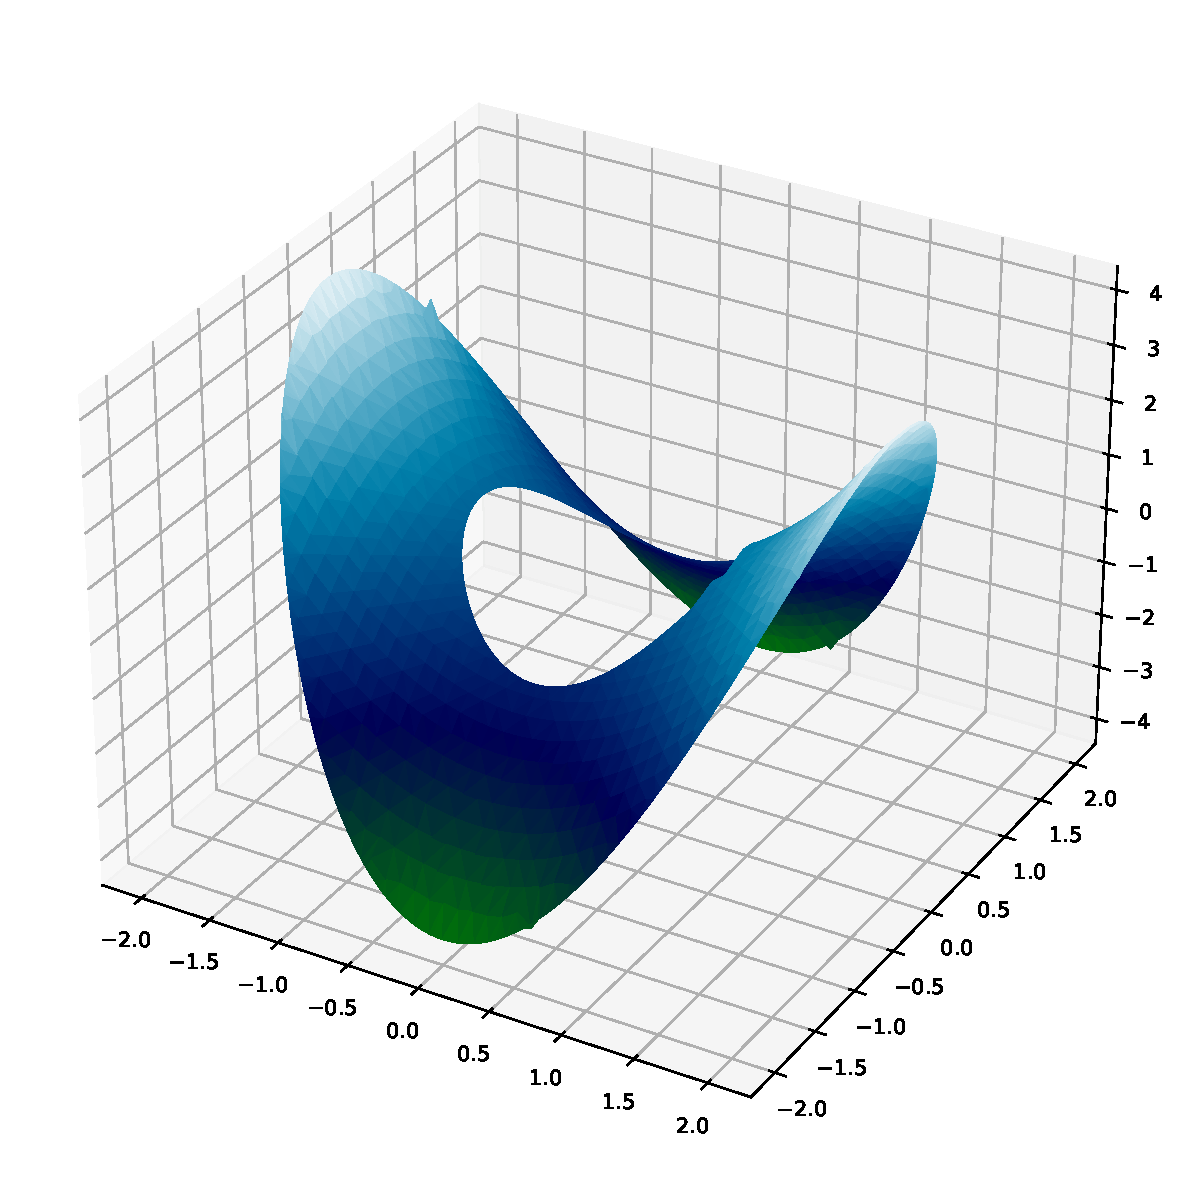
\includegraphics[width=1\textwidth]{resources/ex2-approx.pdf}
	 \caption{Наближений розв'язок}
	\label{fig:ex2-approx}
	 \endminipage
 	\minipage[t]{0.5\textwidth}
 	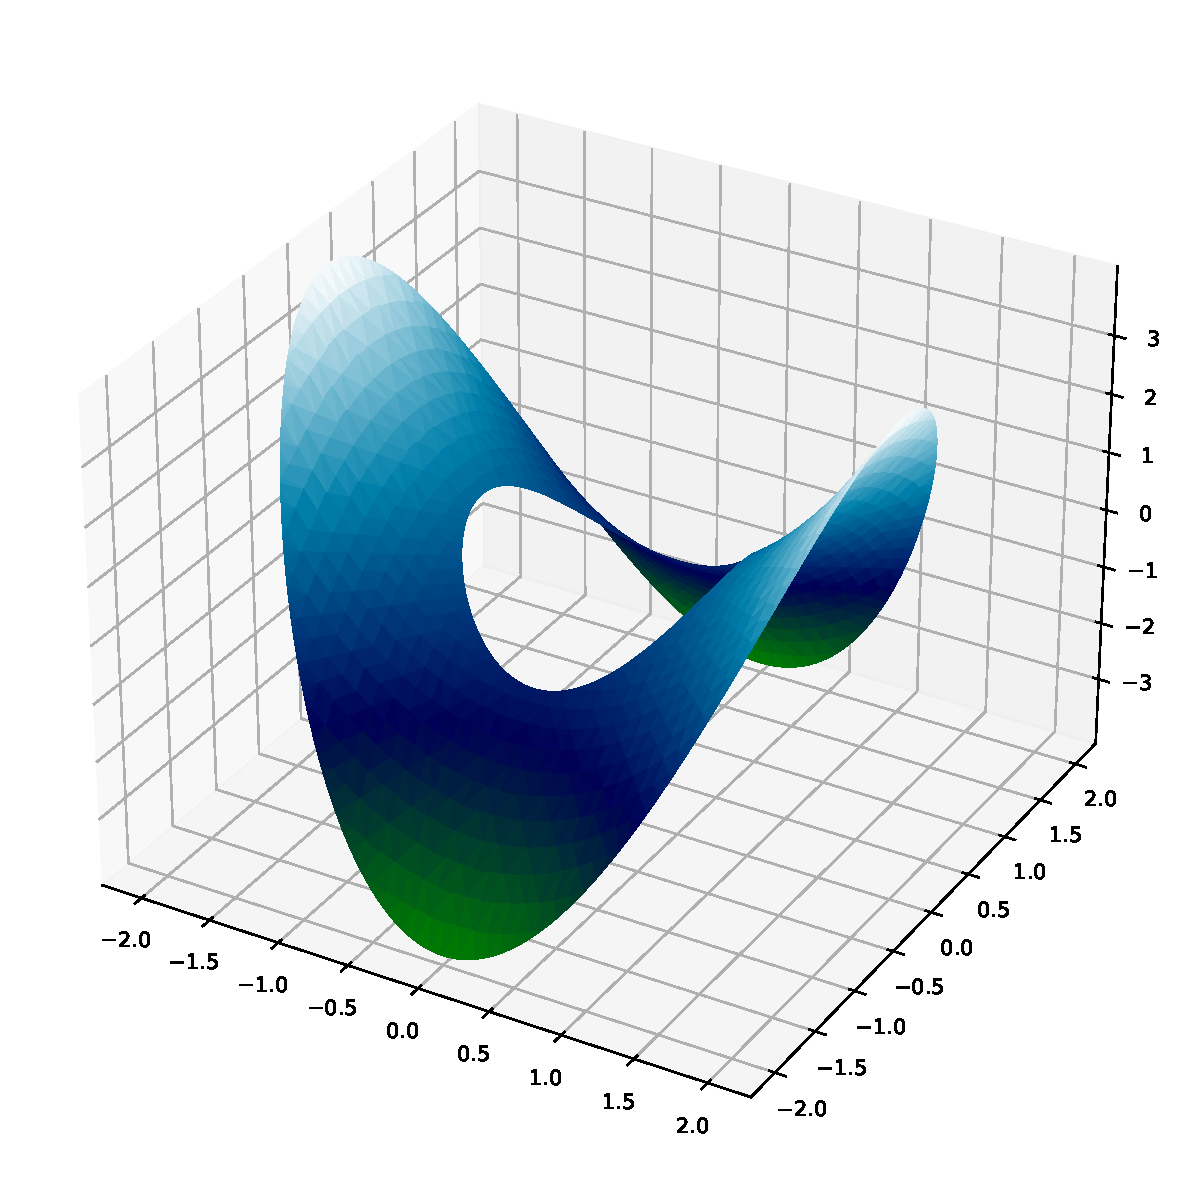
\includegraphics[width=1\textwidth]{resources/ex2-ex.pdf}
 	\caption{Точний розв'язок}	
	\label{fig:ex2-exact}
 	\endminipage\hfill
 \end{figure}

\begin{figure}[!htb]
	\centering
	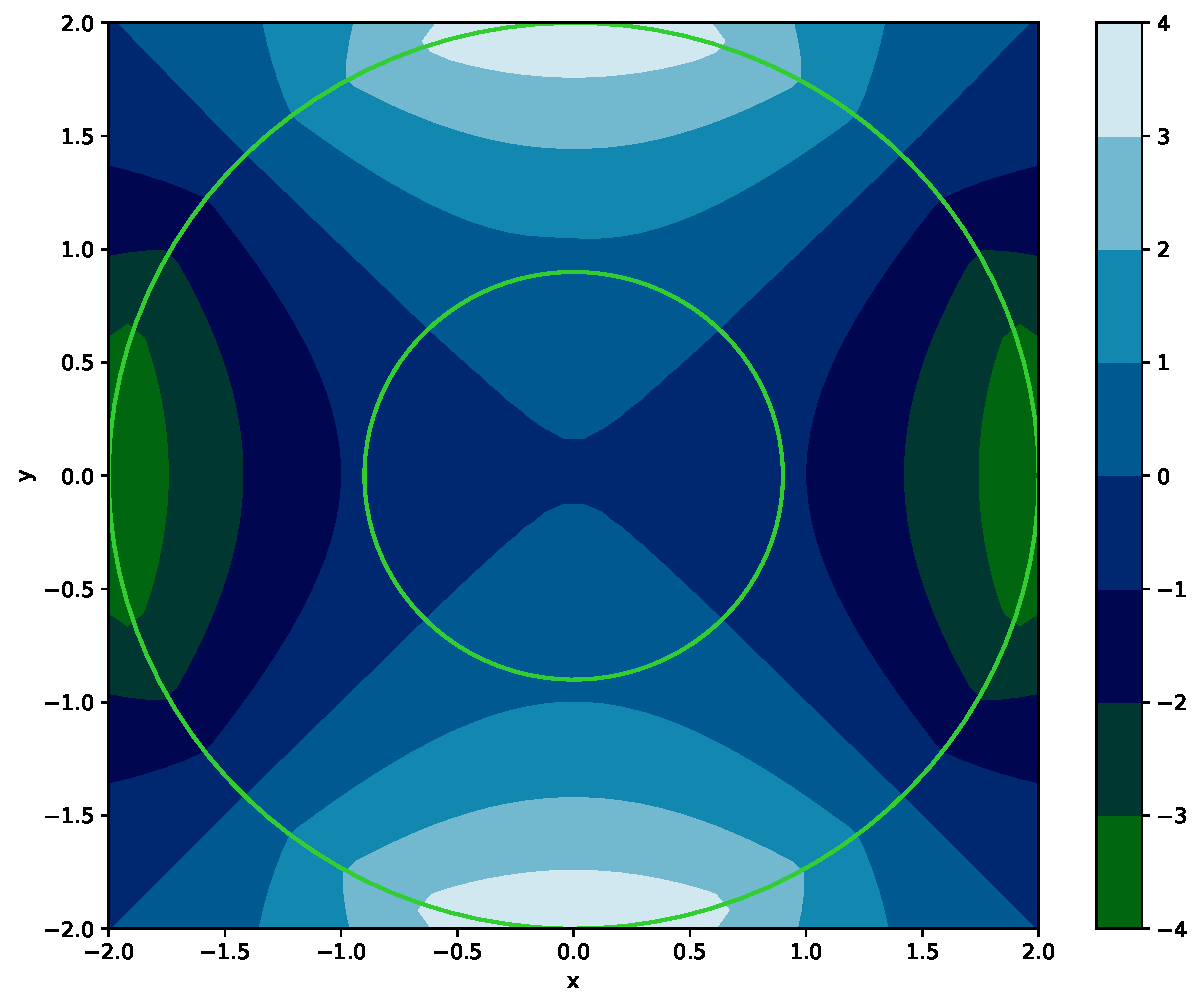
\includegraphics[width=0.45\textwidth]{resources/ex2_contourf.pdf}
	\caption{Лінії рівня наближеного розв'язку}
	\label{fig:ex2_contourf}
\end{figure}

  \newpage
 \thispagestyle{empty}
  \section{Висновок}
	Отже ми розглянули мішану задачу Діріхле-Неймана для рівняння Лапласа у двозв’язній області. Чисельне розв’язування виконано методом колокацій з використання кусково лінійних базисних функцій. Чисельні експерименти підтверджують ефективність методу для розв’язання мішаної задачі для рівняння Лапласа.
	
  
  
 \newpage 
%%%%%%%%%%%%%%%%%%%%%%%%%%%%%%%%%%%%%%%%%%%%%%%%%%%%%%%%%%%%%%%%%%	

\nocite{kress2012linear}
\nocite{chapko2009altrating}
\nocite{chapko2009numerical}
\nocite{atkinson2009}

\printbibliography[title={Бібліографія}]
%%%%%%%%%%%%%%%%%%%%%%%%%%%%%%%%%%%%%%%%%%%%%%%%%%%%%%%%%%%%%%%%%%

\end{document}
 
 